\subsection{Glyphs: \glyph{Units of information for Biological activity}}
\label{sec:af:unitInfo}

When representing biological activities, it is often useful to illustrate the nature of the entity where the activity is originated, e.g., whether the activity is from a macromolecule (protein or nucleic acid), or from a chemical compound.  The \SBGNAFLone \glyph{unit of information} is used to add such information to a glyph.  It represents the information in two ways.  First, different symbols are used to represent the nature of the entity where the activity is from, e.g., macromolecule, nucleic acid feature, or complex.  These symbols are identical to the \glyph{entity pool node} symbols in SBGN \PDl.  Second, names of the entity (gene names, protein names) are usually provided as labels in the \glyph{unit of information} container.

\begin{glyphDescription}

\glyphSboTerm Not applicable.

\glyphContainer A unit of information is represented by containers of different shapes, depending on the nature of the entity where the biological activity is from. There are a total of six types of units of information, as shown in \fig{af:unitInfo}.   Below is a summary of the six glyphs.

\begin{description}
\item[A.] Macromolecule -- Macromolecules are biochemical substances that are built up from the covalent linking of pseudo-identical units. Examples of macromolecules include proteins, nucleic acids (RNA, DNA), and polysaccharides (glycogen, cellulose, starch, etc.).  
A \glyph{macromolecule unit of information} is represented by a rectangle with rounded corners, as illustrated in (A) of \fig{af:unitInfo}.  This container is used to decorate a biological activity that is originated from a macromolecule, such as a protein, a nucleic acid, or a complex sugar.

\item[B.] Nucleic acid feature -- The nucleic acid feature construct in SBGN is meant to represent a fragment of a macromolecule carrying genetic information. A \glyph{nucleic acid feature unit of information} is represented by a rectangle whose bottom half has rounded corners, as shown in (B) of \fig{af:unitInfo}.

\item[C.] Simple chemical -- A simple chemical is a chemical compound that is not formed by the covalent linking of pseudo-identical residues. Examples of simple chemicals are an atom, a monoatomic ion, a salt, a radical, a solid metal, a crystal, etc. 
A \glyph{simple chemical unit of information} is represented by a “stadium” shape, that is two semicircles of the same
radius joined by parallel line segments, as shown in (C) of \fig{af:unitInfo}. If desired the parallel line segments can have zero length, and the shape is then identical to a circle. To avoid confusion with the unspecified entity (shown in D of (\fig{af:unitInfo}), this form of the glyph must remain a circle and cannot be deformed into an ellipse.

\item[D.] Unspecified entity -- An unspecified entity is used to represent the entity type that is unknown or simply not relevant to the purposes of the map. This arises, for example, when the existence of the entity has been inferred indirectly, or when the entity is merely a construct introduced for the needs of a map, without direct biological relevance. An \glyph{unspecified entity unit of information} is represented by an elliptic container, as shown in (D) of \fig{af:unitInfo}.  It is used to decorate a biological activity that is originated from an unspecified entity.

\item[E.] Complex -- A complex represents a biochemical entity composed of other biochemical entities, whether macromolecules, simple chemicals, or other complexes. The resulting entity may 
have its own identity, properties and function in an SBGN map. A \glyph{complex unit of information} is represented by a rectangular shape with cut-corners (that is, an octagonal shape with sides of two different lengths) as shown in (E) of \fig{af:unitInfo}.  It is used to decorate a biological activity that is originated from a complex.

\item[F.] Perturbation -- Biochemical networks can be affected by external influences. Those influences can be well-defined physical perturbations, such as a light pulse or a change in temperature; they can also be more complex and not well-defined phenomena, for instance, glucose deprivation, stress.  A \glyph{perturbation unit of information} is represented by a modified hexagon
having two opposite concave faces, as illustrated in F of  \fig{af:unitInfo}.  It is used to decorate a biological activity when it is originated from a perturbation.
\end{description}

\begin{figure}[H]
  \centering
  \includegraphics[scale = 0.7]{images/build/unit_info_ba_new.pdf}
  \caption{The \AF glyph for \glyph{unit of information}.}
  \label{fig:af:unitInfo}
\end{figure}

\begin{figure}[H]
  \centering
  \includegraphics[scale = 1]{images/build/unit_info_sample.pdf}
  \caption{Examples of \glyph{unit of information} used on \glyph{biological activity node} to indicate that the \emph{Twist-1 activity} is from a \emph{nucleic acid feature} or a \emph{macromolecule}, or a \emph{transcription factor activity} from an \emph{unspecified} entity.}
  \label{fig:af:unitofinfo}
\end{figure}

\fig{af:unitofinfo} shows examples taken from \fig{af:1}, where \emph{units of information} are used on \glyph{biological activities} to illustrate the nature of the entities from which the activities originate.

The long side of the glyphs above must be orientated parallel to the border of the biological activity being annotated by the unit of information. The centre of the bounding box of a unit of information must lie on the border of the \glyph{BA}.

\glyphLabel A \glyph{unit of information} is not required to carry any label.   If a label is desired, it must be placed in an unbordered box containing a string of characters. The characters can be distributed on several lines to improve readability, although this is not mandatory.  The label box must be attached to the centre of the container. The label may spill outside of the container.  The label defines the information carried by the \glyph{unit of information}.

\glyphAux None.

\end{glyphDescription}

\subsection{Glyph: \glyph{Unit of information for Compartment}}
\label{sec:af:unitInfoComp}

A \emph{unit of information} can be used to decorate a compartment to convey information about physical characteristics of the compartments (\sect{af:physical-characteristics-cv}). 

\begin{glyphDescription}

\glyphSboTerm Not applicable.

\glyphContainer A \emph{unit of information} for a compartment is represented by a rectangle as shown in \fig{compunitInfo}.  The long side of the rectangle must be orientated parallel to the border of the \glyph{compartment} being annotated by the \glyph{unit of information}. The centre of the bounding box of a \glyph{unit of information} must lie on the border of the \glyph{compartment}.

\begin{figure}[H]
  \centering
  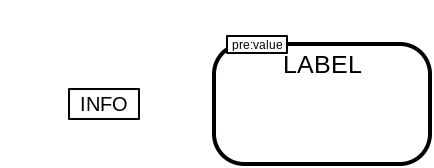
\includegraphics[scale = 0.7]{images/build/unit_info_comp.pdf}
  \caption{The \AF glyph for \glyph{unit of information}, shown plain on the left, and decorating a \glyph{compartment} (\sect{compartment}) on the right.}
  \label{fig:compunitInfo}
\end{figure}

\glyphLabel A \glyph{unit of information} is identified by a label placed in an unbordered box containing a string of characters.  The characters can be distributed on several lines to improve readability, although this is not mandatory.  The label box must be attached to the centre of the container.  The label may spill outside of the container. The label defines the information carried by the \glyph{unit of information}. The controlled vocabularies predefined in \SBGNAFLone for \glyph{unit of information}, regarding compartments, are described in \sect{af:physical-characteristics-cv}.
    
\glyphAux None. 

\end{glyphDescription}


